\begin{frame}
  \begin{PointSix}{Houskeeping}
    \begin{itemize}
      \item \alert{Geophysics at seminar 20.05.2022}
      \item \alert{Questions regarding exercises}
    \end{itemize}
  \end{PointSix}
\end{frame}

\begin{frame}
  \begin{PointSix}{Learning Goals}
    \begin{itemize}
      \item \alert{Resistivity..}
      \item \alert{Currents..}
      \item \alert{Electric Fields..}
    \end{itemize}
  \end{PointSix}
\end{frame}

\begin{frame}
  \begin{PointSix}{Resistivity Method Principles}
      \small
      Characterize the sub-surface in it's ability to conduct electrical currents. A material that has a high electrical resistivity will conduct electrical currents poorly and vice versa.
  \end{PointSix}
\end{frame}

\begin{frame}
  \begin{PointSix}{Primary parameter of the resistivity method}
   % RESISTOR with battery and arrow

    \begin{tikzpicture}
      
      \newcommand\EMF{\mathcal{E}};
      \colorlet{Icol}{blue!50!black}
      \colorlet{Ccol}{orange!90!black}
      \colorlet{Rcol}{Karminrot}
      \colorlet{loopcol}{red!90!black!25}
      \colorlet{pluscol}{red!60!black}
      \colorlet{minuscol}{blue!60!black}
      \tikzstyle{EMF}=[battery1,l=$\EMF$];
      \tikzstyle{internal R}=[R,color=Rcol,Rcol,l=$r$,/tikz/circuitikz/bipoles/length=30pt];
      \tikzstyle{loop}=[->,red!90!black!25];
      \tikzstyle{loop label}=[loopcol,fill=white,scale=0.8,inner sep=1];
      \tikzstyle{thick R}=[R,color=Rcol,thick,Rcol,l=$R$];
      
      \begin{scope}[rotate=-90,transform shape]
        \fill[pattern = crosshatch dots,pattern color = brown!80!red] (0.5,-0.5) rectangle ++(6,9);
        \node[rotate=90] at (0.25,1.5) {Surface};
        \draw (0,8) to [short,*-] (4,8) to[R,color=Rcol,thick,l={{{{\rotatebox[origin=c]{90}{$R$}}}}}] (4,0) to [short,-*] (0,0);
        \node[rotate=90,above] at (0,8) {$+$};
        \node[rotate=90,above] at (0,0) {$-$};
        \node[rotate=90] at (0,4) {$\Delta V$};
          %  \draw[->,red] (0.5, 2.15) --++ (1.2,0) node[midway,above=1] {current $I$};
          %  \draw[->,red] (0.5,-0.15) --++ (1.2,0) node[midway,below=1] {electron flow};
          \end{scope}
    \end{tikzpicture}
  \end{PointSix}
\end{frame}

\begin{frame}
     \begin{PointSix}{Resistivity vs. Resistance}
      \begin{center}
        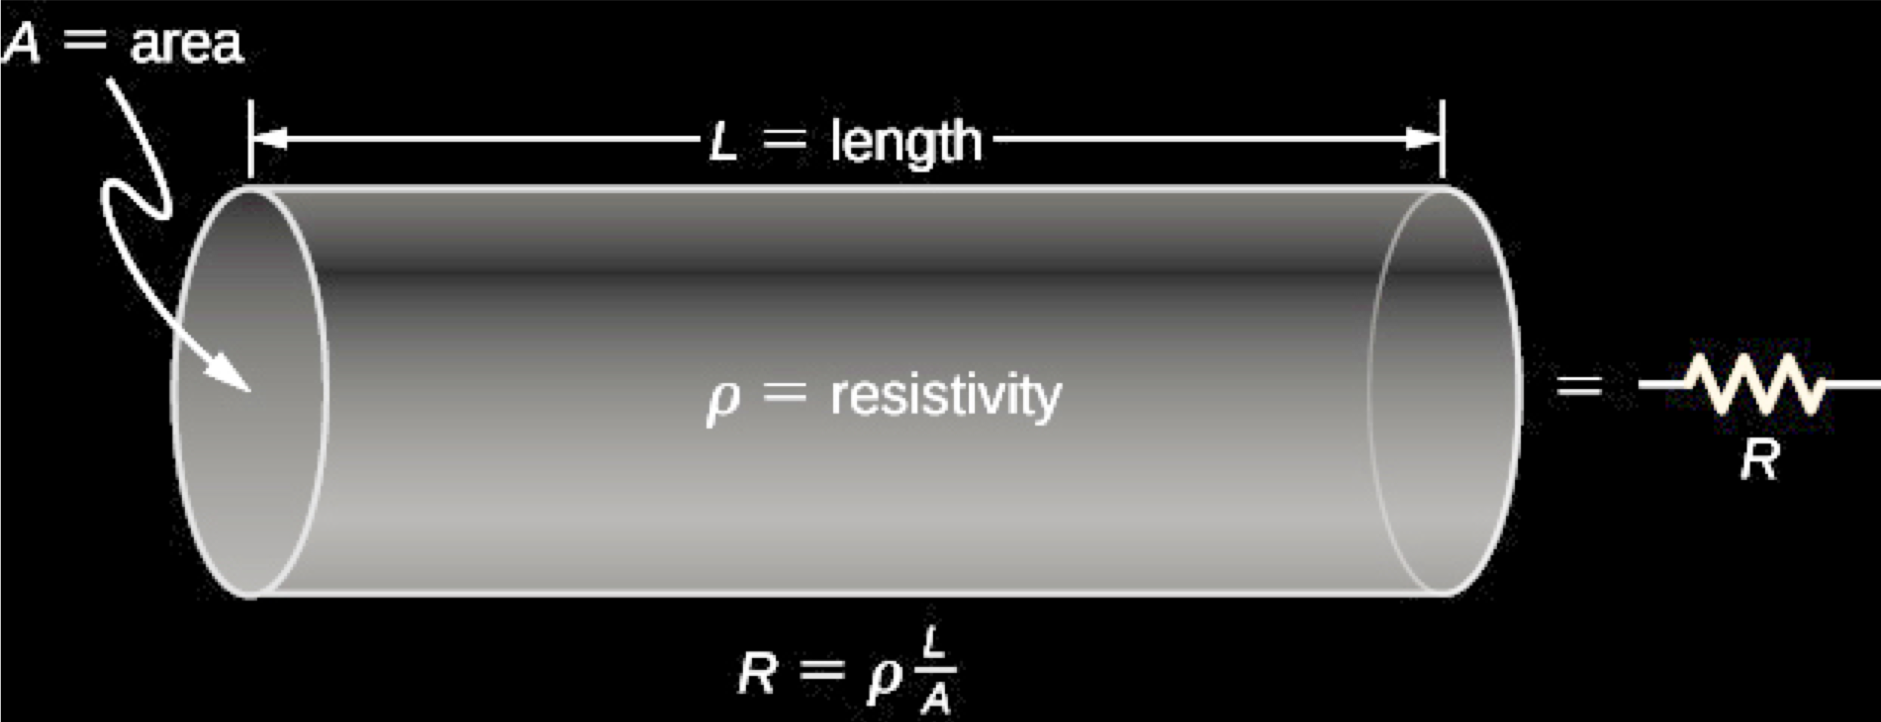
\includegraphics[width=0.90\linewidth]{Figures/Resistivity/ResistanceResistivity.png}
      \end{center}
      \small
      \begin{itemize}
        \item Resistivity (spez. elektr. Widerstand) is a material property
        \item Resistance (elektr. Widerstand) includes material and geometry of the resistor
      \end{itemize}
      \end{PointSix}
\end{frame}

\begin{frame}
  \begin{PointSix}{Resistivity vs. Resistance}
   \begin{center}
     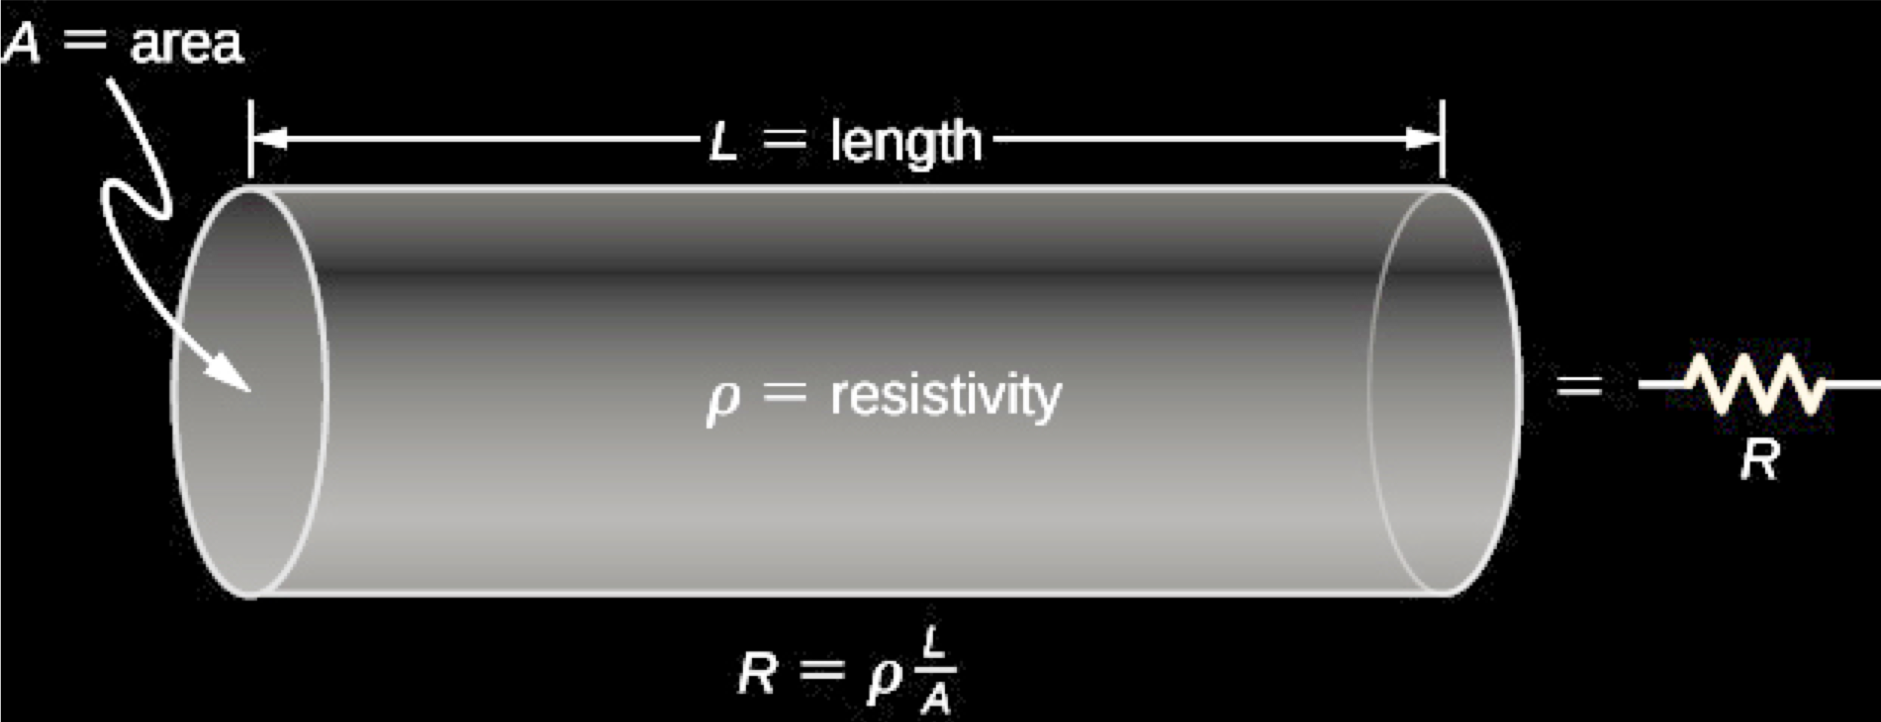
\includegraphics[width=0.90\linewidth]{Figures/Resistivity/ResistanceResistivity.png}
   \end{center}
   \small
   \begin{itemize}
     \item Resistance [Ohm, $\Omega$]
     \item Resistivity [$\Omega m$]
   \end{itemize}
   \end{PointSix}
\end{frame}

\begin{frame}
  \begin{PointSix}{Resistivity ($\rho$) vs. Conductivity ($\sigma$)}
   \begin{center}
     $$
      \rho = \frac{1}{\sigma}
     $$
   \end{center}
   \small
   \begin{itemize}
     \item Resistivity [$\Omega m$]
     \item Conductivity [$(\Omega m)^{-1}$, i.e. Siemens]
   \end{itemize}
   \end{PointSix}
\end{frame}

\begin{frame}
  \begin{PointSix}{Ionic vs. metallic conduction}
    \begin{center}
      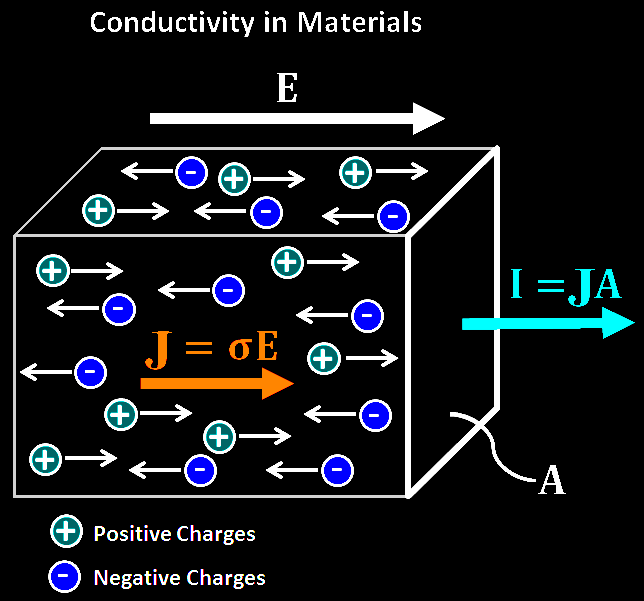
\includegraphics[width=0.80\linewidth]{Figures/Resistivity/conductivity_physics_diagram_RGeoSciXYZ.png}
      \tiny[GeoSci XYZ]
    \end{center}
   
      
  \end{PointSix}
\end{frame}

\begin{frame}
  \begin{PointSix}{Ionic vs. metallic}
    \begin{center}
      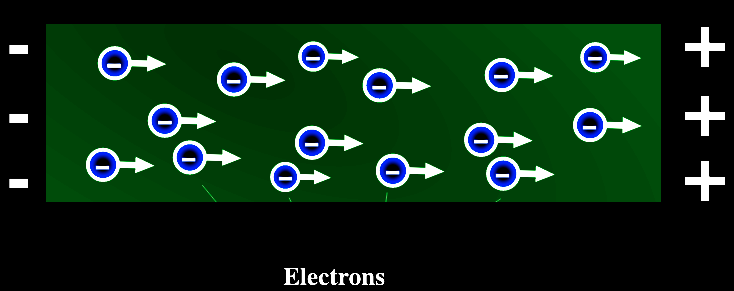
\includegraphics[width=0.90\linewidth]{Figures/Resistivity/MetallicCondution.png}
     % \tiny[GeoSci XYZ]
    \end{center}
    \small
    \begin{itemize}
      \item \alert{Metallic conduction} uses declocalized electrons in the conduction band of metalls
      \item \alert{Ionic conduction} uses charged Ions in electrolyt 
    \end{itemize}
    \end{PointSix}
\end{frame}
\begin{frame}
  \begin{PointSix}{Ionic conduction in porous sediments}
    \begin{center}
      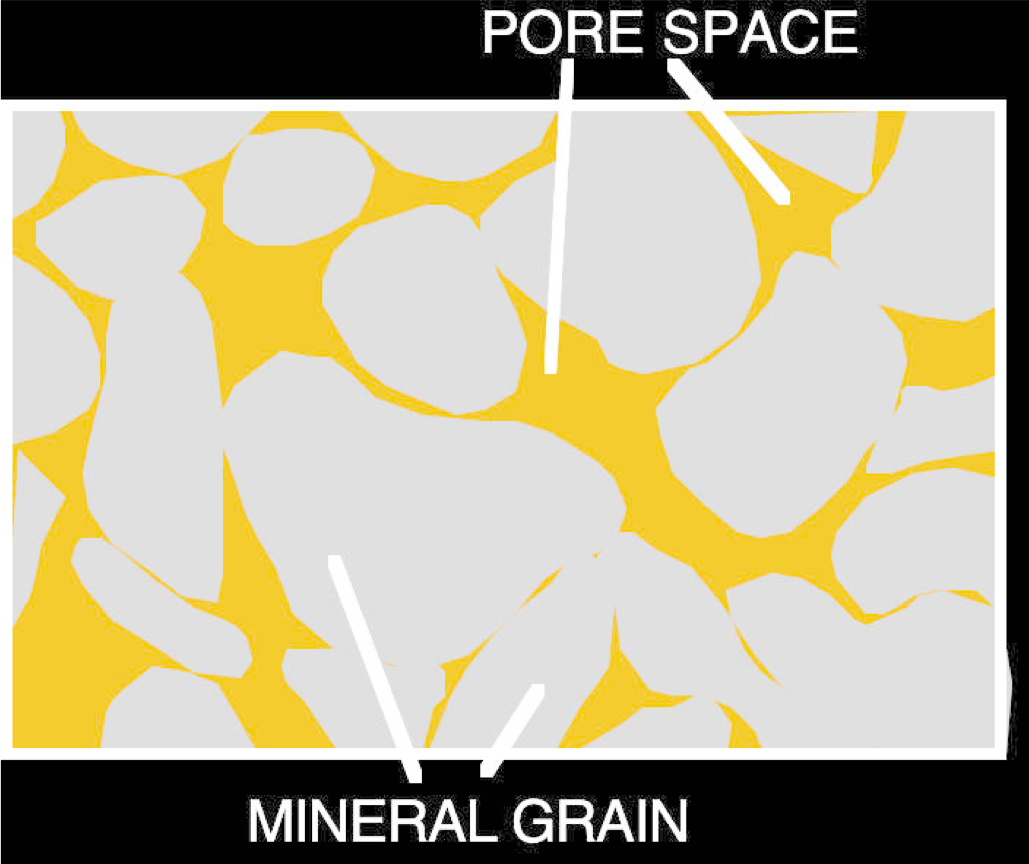
\includegraphics[width=0.90\linewidth]{Figures/Resistivity/ProusMedia.png}
     % \tiny[GeoSci XYZ]
    \end{center}
    \end{PointSix}
\end{frame}

\begin{frame}
  \begin{PointSix}{Ionic conduction in porous sediments}
    \small
    \begin{itemize}
      \item Increases with increasing pore space ($\phi$)
      \item Increases with increasing water saturation
      \item Increases with decreasing water resistivity ($\rho$)
    \end{itemize}
    \normalsize
    \onslide<2>{
      \begin{equation}
        \rho_t = a\rho_w\phi^{-m}s_w^{-n}
      \end{equation}
      \begin{center}
       \small (Archie's Law)
      \end{center}
      
      }
    \end{PointSix}
\end{frame}

\begin{frame}
 % \begin{PointSix}{Huge spread in material properties}
   % RESISTOR with battery and arrow
   \begin{center}
    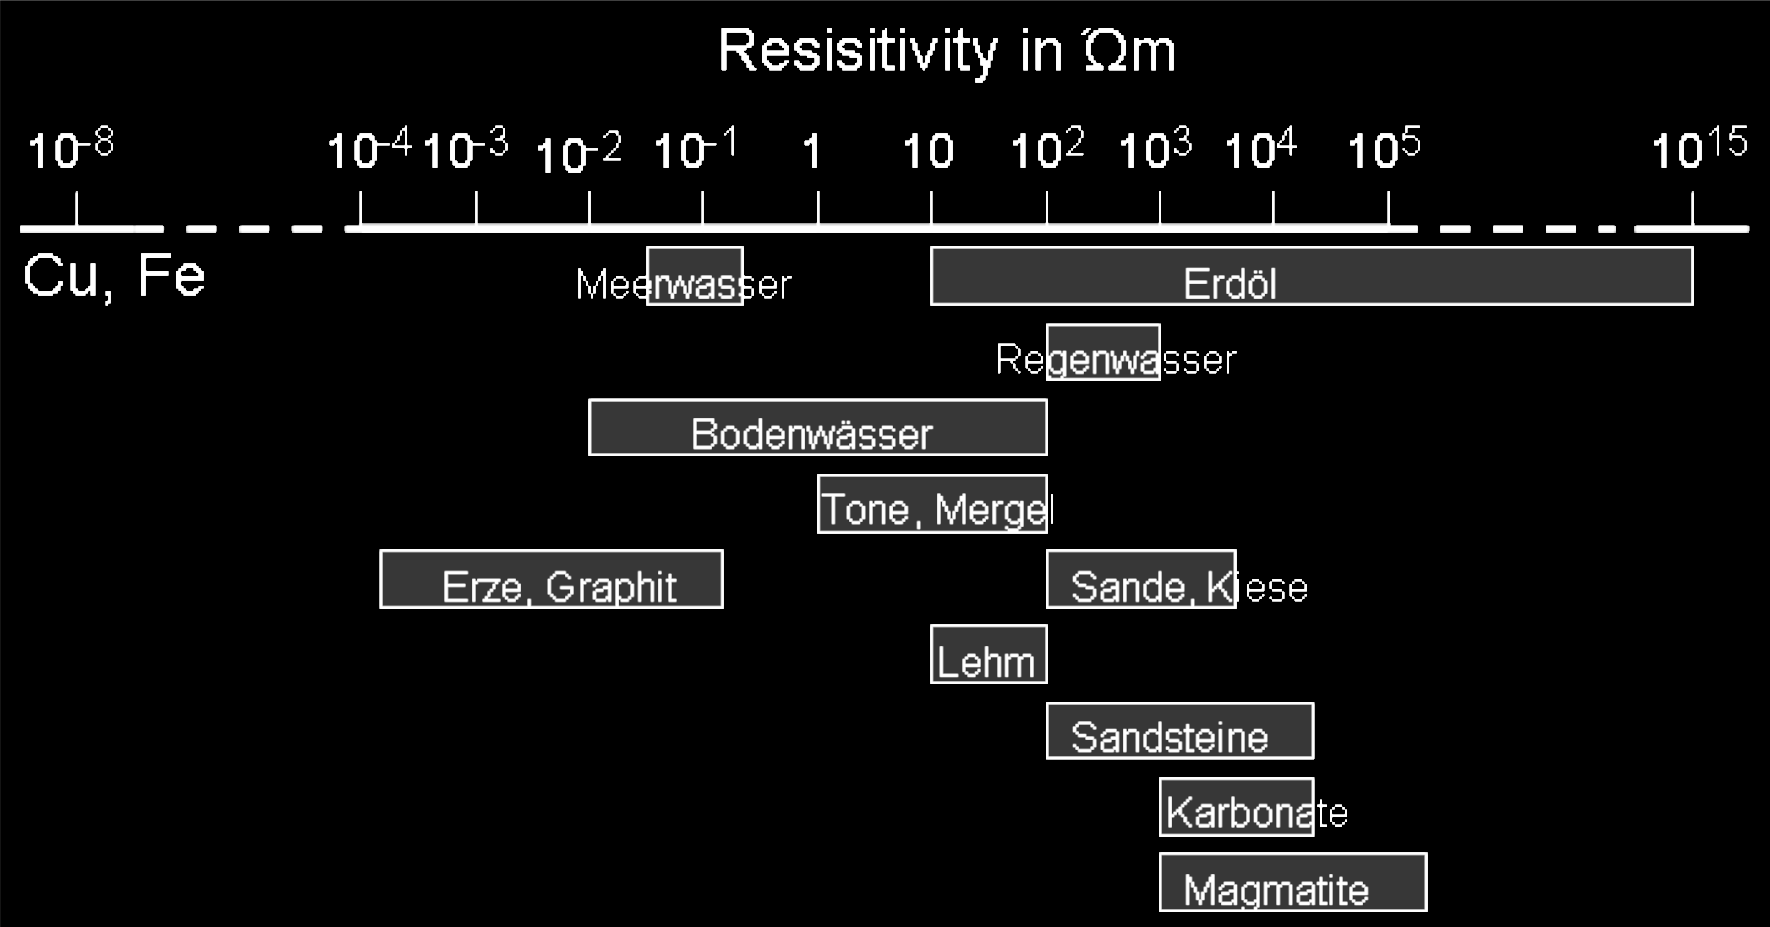
\includegraphics[width=0.8\linewidth]{Figures/Resistivity/ResistivityMaterials.png}
    
  \end{center}
  %\end{PointSix}
\end{frame}

\begin{frame}{Current flow through the sub-surface}
  \begin{PointSix}{Current flow through the sub-surface}
    \small
    Consider a homogeneous conducting halfspace, with constant resistivity $\rho$, under an insulating medium. Let there be a point electrode at the surface
injecting a steady current I. The current flows to a distributed sink at infinity. Find the electrostatic potential, the electric field, and consequently the pattern of current flow in the sub-surface.

    [cf. Telford Chapter 8, online resources resistivity 1 and resistivity 2.]
  \end{PointSix}
\end{frame}

\begin{frame}{Current flow through the sub-surface}
  \begin{PointSix}{Primary parameter of the resistivity method}
   % RESISTOR with battery and arrow
   \begin{center}
    \begin{tikzpicture}
      \coordinate (A) at (8,0);
      \coordinate (B) at (4,-0.5);
      \coordinate (C) at (5,-3.5);
      \coordinate (D) at (6,-3.5);
      \draw [thick] (0,0.0) -- (8,0.0);
      % drawing the node with shape=rectangle and anchor=center
      %\node [draw, Karminrot, thick, shape=rectangle, minimum width=0.25cm, minimum height=0.25cm, anchor=center] at (B) {};
      \draw [->, line width = 1mm] (4,0.5) -- (B) node[xshift=1.0cm,yshift=1.0cm,midway,left] {current $\vec{I}$};;
  
      \node[yshift=0.3cm] at (A) {\small Surface};
  
    \end{tikzpicture}
    % $$
    %   \boxed{\vec{j} = \sigma \vec{E}}
    % $$
    % \small
    % $\vec{E}$ is the electrical field ($V m^{-1}$ )\\
    % $\vec{j}$ is the current density ($A m^{-2}$) \\
    % \vspace{1cm}
    % \alert{Currents flow parallel to the electrical field.}
  \end{center}
  \end{PointSix}
\end{frame}

\begin{frame}
  \begin{PointSix}{Current flow through the sub-surface}
   % RESISTOR with battery and arrow
   \begin{center}
    \begin{tikzpicture}
      \coordinate (A) at (8,0);
      \coordinate (B) at (4,-0.5);
      \coordinate (C) at (5,-3.5);
      \coordinate (D) at (6,-3.5);
      \draw [thick] (0,0.0) -- (8,0.0);
      % drawing the node with shape=rectangle and anchor=center
      %\node [draw, Karminrot, thick, shape=rectangle, minimum width=0.25cm, minimum height=0.25cm, anchor=center] at (B) {};
      \draw [->, line width = 1mm] (4,0.5) -- (B) node[xshift=1.0cm,yshift=1.0cm,midway,left] {current $\vec{I}$};;
  
      \node[yshift=0.3cm] at (A) {\small Surface};
  
    \end{tikzpicture}
    $$
      \boxed{\vec{j} = \sigma \vec{E}}
    $$
    \small
    $\vec{E}$ is the electrical field ($V m^{-1}$ )\\
    $\vec{j}$ is the current density ($A m^{-2}$) \\
    \vspace{1cm}
    \alert{Currents flow parallel to the electrical field.}
  \end{center}
  \end{PointSix}
\end{frame}

\begin{frame}
  \begin{PointSix}{Current flow through the sub-surface}
   % RESISTOR with battery and arrow
   \begin{center}
    \begin{tikzpicture}
      \coordinate (A) at (8,0);
      \coordinate (B) at (4,-0.5);
      \coordinate (C) at (5,-3.5);
      \coordinate (D) at (6,-3.5);
      \draw [thick] (0,0.0) -- (8,0.0);
      % drawing the node with shape=rectangle and anchor=center
      %\node [draw, Karminrot, thick, shape=rectangle, minimum width=0.25cm, minimum height=0.25cm, anchor=center] at (B) {};
      \draw [->, line width = 1mm] (4,0.5) -- (B) node[xshift=1.0cm,yshift=1.0cm,midway,left] {current $\vec{I}$};;
  
      \node[yshift=0.3cm] at (A) {\small Surface};
  
    \end{tikzpicture}
    $$
      \vec{j} = \sigma \vec{E} = \sigma \nabla \phi
    $$
    \small
    %\vspace{1cm}
    \alert{The electrical field is perpendicular to the electric potential (Volts).}
  \end{center}
  \end{PointSix}
\end{frame}

\begin{frame}
  \begin{PointSix}{Current flow through the sub-surface}
   % RESISTOR with battery and arrow
   \begin{center}
    \begin{tikzpicture}
      \coordinate (A) at (8,0);
      \coordinate (B) at (4,-0.5);
      \coordinate (C) at (5,-3.5);
      \coordinate (D) at (6,-3.5);
      \draw [thick] (0,0.0) -- (8,0.0);
      % drawing the node with shape=rectangle and anchor=center
      %\node [draw, Karminrot, thick, shape=rectangle, minimum width=0.25cm, minimum height=0.25cm, anchor=center] at (B) {};
      \draw [->, line width = 1mm] (4,0.5) -- (B) node[xshift=1.0cm,yshift=1.0cm,midway,left] {current $\vec{I}$};;
  
      \node[yshift=0.3cm] at (A) {\small Surface};
  
    \end{tikzpicture}
    $$
      \nabla\cdot\vec{j} = 0
    $$
    \small
    %\vspace{1cm}
    \alert{In the half space there are no sources and sinks for the current density. Understand this from what we learned about the magnetic dipole field which is also divergence free.}
  \end{center}
  \end{PointSix}
\end{frame}



\begin{frame}
  \begin{PointSix}{Current flow through the sub-surface}
   % RESISTOR with battery and arrow
   \begin{center}
    \begin{tikzpicture}
      \coordinate (A) at (8,0);
      \coordinate (B) at (4,-0.5);
      \coordinate (C) at (5,-3.5);
      \coordinate (D) at (6,-3.5);
      \draw [thick] (0,0.0) -- (8,0.0);
      % drawing the node with shape=rectangle and anchor=center
      %\node [draw, Karminrot, thick, shape=rectangle, minimum width=0.25cm, minimum height=0.25cm, anchor=center] at (B) {};
      \draw [->, line width = 1mm] (4,0.5) -- (B) node[xshift=1.0cm,yshift=1.0cm,midway,left] {current $\vec{I}$};;
  
      \node[yshift=0.3cm] at (A) {\small Surface};
  
    \end{tikzpicture}
    $$
    \nabla \cdot \vec{j} = \sigma \nabla \cdot \vec{E} = \sigma \nabla^2 \phi =0
    $$
    \small
    %\vspace{1cm}
    \alert{This is the Laplace equation.}
  \end{center}
  \end{PointSix}
\end{frame}

\begin{frame}
  \begin{PointSix}{Current flow through the sub-surface}
   % RESISTOR with battery and arrow
   \begin{center}
    \begin{tikzpicture}
      \coordinate (A) at (8,0);
      \coordinate (B) at (4,-0.5);
      \coordinate (C) at (5,-3.5);
      \coordinate (D) at (6,-3.5);
      \draw [thick] (0,0.0) -- (8,0.0);
      % drawing the node with shape=rectangle and anchor=center
      %\node [draw, Karminrot, thick, shape=rectangle, minimum width=0.25cm, minimum height=0.25cm, anchor=center] at (B) {};
      \draw [->, line width = 1mm] (4,0.5) -- (B) node[xshift=1.0cm,yshift=1.0cm,midway,left] {current $\vec{I}$};;
  
      \node[yshift=0.3cm] at (A) {\small Surface};
  
    \end{tikzpicture}
    \begin{eqnarray*}
    &\nabla \cdot \vec{j} = \sigma \nabla \cdot \vec{E} = \sigma \nabla^2 \phi =0 \\
    &\rightarrow \phi = \frac{A}{r}
    \end{eqnarray*}
    \small
    %\vspace{1cm}
    (Exercises)\\
    \alert{The current flows radially outwards.}
  \end{center}
  \end{PointSix}
\end{frame}

\begin{frame}
  \begin{PointSix}{Current flow through the sub-surface}
   % RESISTOR with battery and arrow
   \begin{center}
    \begin{tikzpicture}
      \coordinate (A) at (8,0);
      \coordinate (B) at (4,-0.5);
      \coordinate (C) at (5,-3.5);
      \coordinate (D) at (6,-3.5);
      \draw [thick] (0,0.0) -- (8,0.0);
      % drawing the node with shape=rectangle and anchor=center
      %\node [draw, Karminrot, thick, shape=rectangle, minimum width=0.25cm, minimum height=0.25cm, anchor=center] at (B) {};
      \draw [->, line width = 1mm] (4,0.5) -- (B) node[xshift=1.0cm,yshift=1.0cm,midway,left] {current $\vec{I}$};;
  
      \node[yshift=0.3cm] at (A) {\small Surface};
  
    \end{tikzpicture}
    \begin{eqnarray*}
    I &=& 2\pi r^2 j \\   
      &=& -2\pi r^2 \sigma \nabla \phi \\
      &=& 2\pi \sigma A
    \end{eqnarray*}
    $$
    A = -\frac{I\rho}{4\pi}
    $$
    \small
  \end{center}
  \end{PointSix}
\end{frame}

\begin{frame}
  \begin{PointSix}{Current flow through the sub-surface}
   % RESISTOR with battery and arrow
   \begin{center}
    \begin{tikzpicture}
      \coordinate (A) at (8,0);
      \coordinate (B) at (4,-0.5);
      \coordinate (C) at (5,-3.5);
      \coordinate (D) at (6,-3.5);
      \draw [thick] (0,0.0) -- (8,0.0);
      % drawing the node with shape=rectangle and anchor=center
      %\node [draw, Karminrot, thick, shape=rectangle, minimum width=0.25cm, minimum height=0.25cm, anchor=center] at (B) {};
      \draw [->, line width = 1mm] (4,0.5) -- (B) node[xshift=1.0cm,yshift=1.0cm,midway,left] {current $\vec{I}$};;
  
      \node[yshift=0.3cm] at (A) {\small Surface};
  
    \end{tikzpicture}
    $$
      \boxed{\phi = \frac{I\rho}{2\pi} \frac{1}{r}}
    $$
    \small
  \end{center}
  \end{PointSix}
\end{frame}


\begin{frame}{Current flow through the sub-surface}
  % \begin{PointSix}{Primary parameter of the resistivity method}
    % RESISTOR with battery and arrow
    \begin{center}
     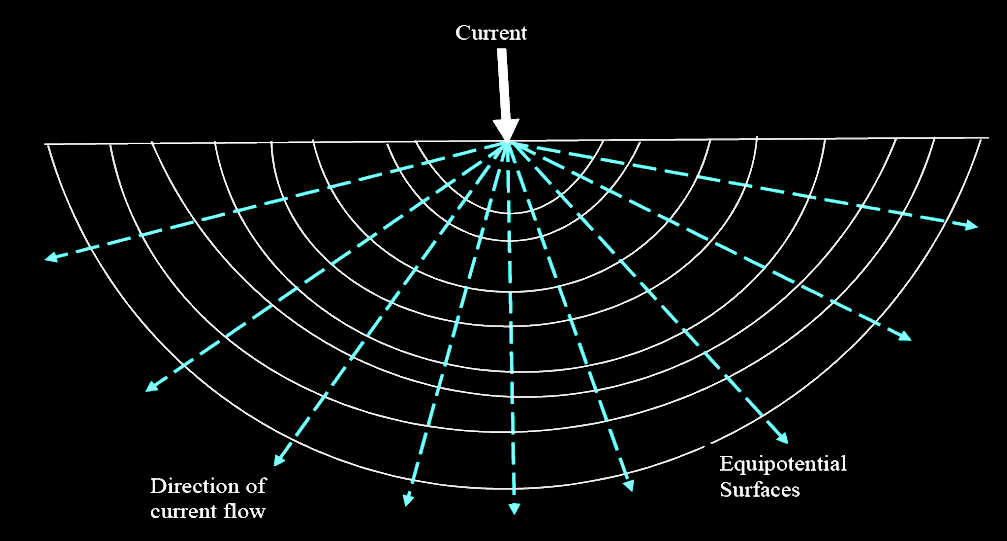
\includegraphics[width=0.7\linewidth]{Figures/Resistivity/OneElectrodeHomoHalfspace_Aizebeokhai_SResanEss2010.png}
 
     \tiny[Aizebeokhai et al., 2010]
   \end{center}
   %\end{PointSix}
 \end{frame}


